
\section*{Question 3}

\begin{enumerate}[(a)]
    \item
    N=840\\
    \begin{figure}[h]
        \centering
        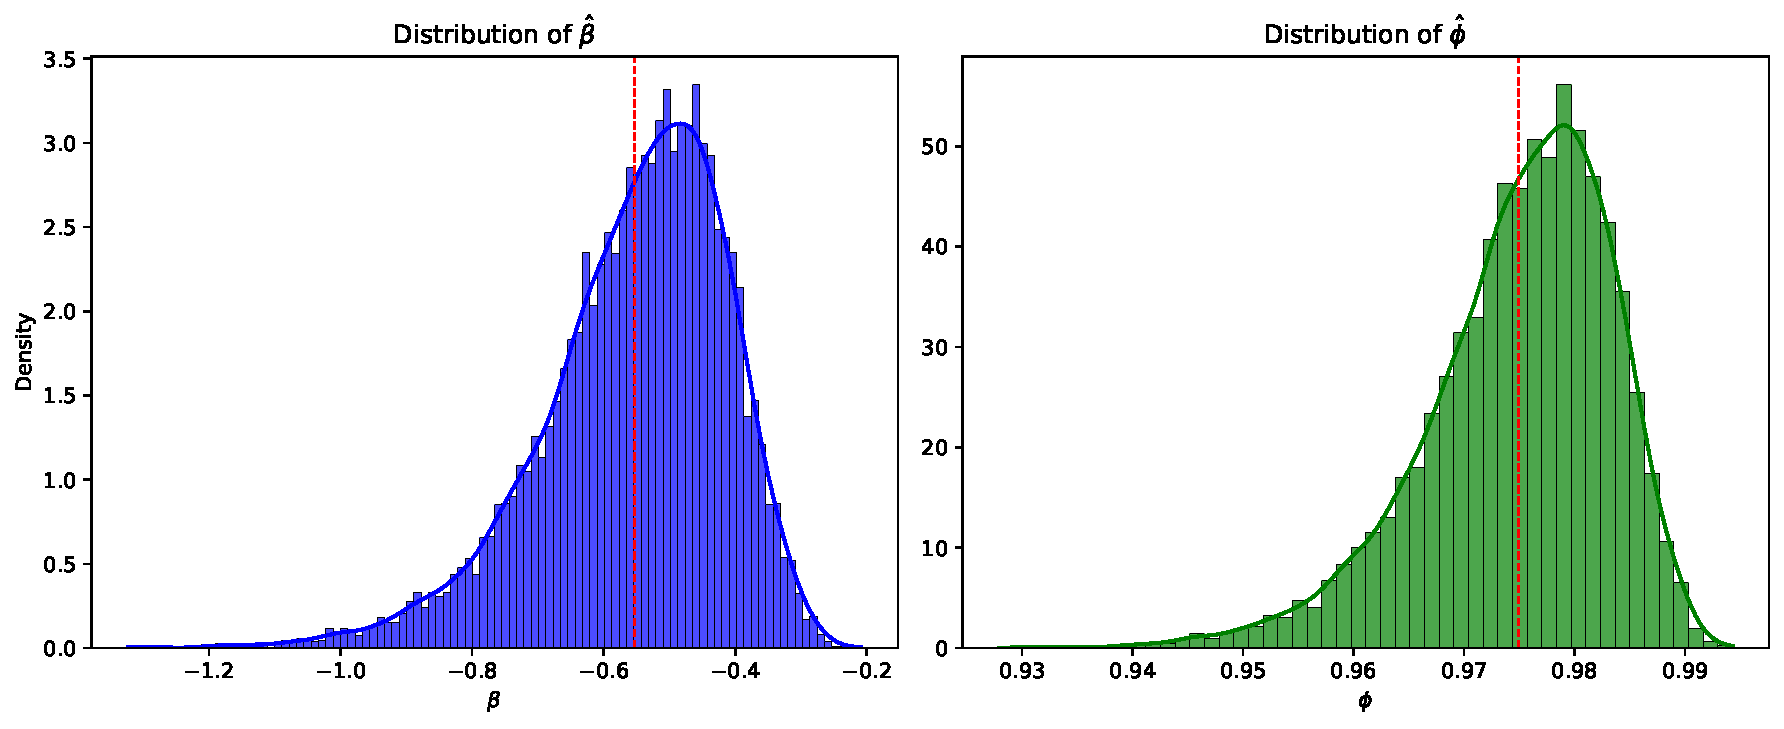
\includegraphics[width=0.9\linewidth]{Out/EX3-1.pdf}
        
    \end{figure}

  \item
    N=240\\
    \begin{figure}[h]
        \centering
        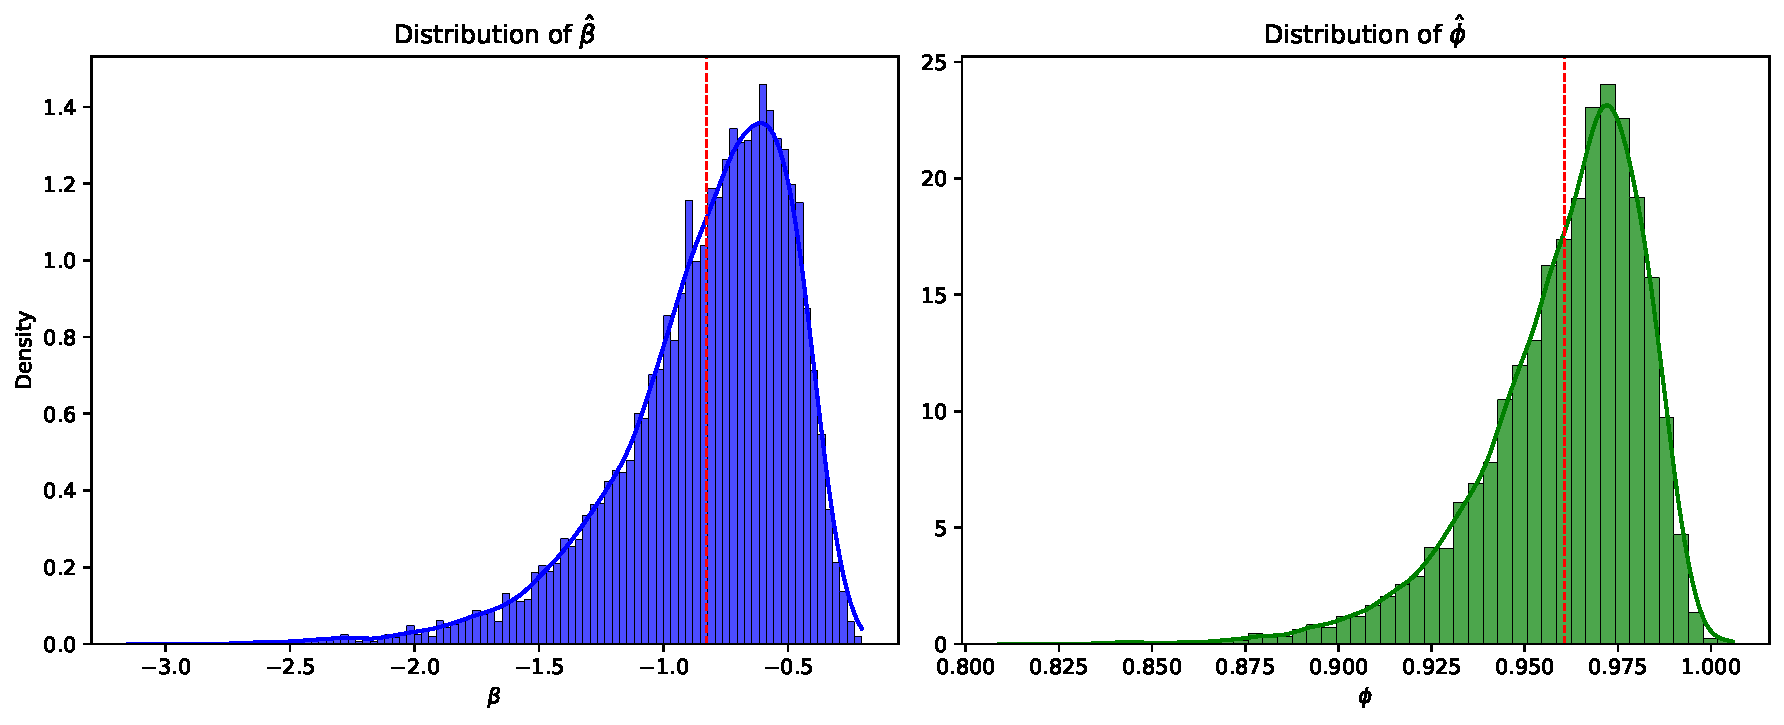
\includegraphics[width=0.9\linewidth]{Out/EX3-2.pdf}
        
    \end{figure}
Compared with the estimation with n=840, the estimation with n=240 is more biased, it's more skewed to the right side and away from the true value.
\item 
We rejected 0 times out of 10,000 when when assuming IID errors, 
suggesting that we reject the null hypothesis. 
However, we should be expecting high rejection rate since the real value of beta is 0.\\
This difference might be due to the fact that the errors are not independent.\\

\item 
We rejected 9.77\% of the simulations out of 10,000 runs when using Newey-West standard errors, suggesting that there is autocorrelation present in the errors, and the standard errors are adjusted to account for this.\\

\end{enumerate}

